\documentclass[11pt]{article}

\usepackage{amsmath, amssymb, amsthm}
\usepackage{tikz}

\theoremstyle{plain}
\newtheorem{thm}{Theorem}[section]
\newtheorem*{thm*}{Theorem}
\newtheorem{prop}[thm]{Proposition}
\newtheorem{lem}[thm]{Lemma}
\newtheorem*{lem*}{Lemma}
\newtheorem{dfn}[thm]{Definition}
\newtheorem{cor}[thm]{Corollary}
\newtheorem{claim}[thm]{Claim}
\newtheorem{conj}[thm]{Conjecture}
\newtheorem{ques}[thm]{Question}
\newtheorem*{rem}{Remark}


\oddsidemargin  0pt
\evensidemargin 0pt
\marginparwidth 40pt
\marginparsep 10pt
\topmargin 0pt
\headsep 10pt
\textheight 8.2in
\textwidth 6.4in
\renewcommand{\baselinestretch}{1.1}

\newcommand{\codeg}{\text{codeg}}
\newcommand{\BBE}{\mathbb{E}}
\newcommand{\BFP}{\mathbf{P}}
\usepackage{amsmath}
\usepackage{amsthm}
\usepackage{amssymb}
\usepackage{mathtools}
\usepackage{hyperref}
\usepackage{url}





\usepackage{graphicx}
\usepackage{caption}
\usepackage{subcaption}

\def\eQb#1\eQe{\begin{eqnarray*}#1\end{eqnarray*}}
\def\eQnb#1\eQne{\begin{eqnarray}#1\end{eqnarray}}
\providecommand{\e}[1]{\ensuremath{\times 10^{#1}}}
\providecommand{\pb}[0]{\pagebreak}
\DeclarePairedDelimiter\ceil{\lceil}{\rceil}
\DeclarePairedDelimiter\floor{\lfloor}{\rfloor}

\newcommand{\E}{\mathrm{E}}
\newcommand{\Var}{\mathrm{Var}}
\newcommand{\Cov}{\mathrm{Cov}}

\def\Qb#1\Qe{\begin{question}#1\end{question}}
\def\Sb#1\Se{\begin{solution}#1\end{solution}}


\newtheoremstyle{quest}{\topsep}{\topsep}{}{}{\bfseries}{}{ }{\thmname{#1}\thmnote{ #3}.}
\theoremstyle{quest}
\newtheorem*{definition}{Definition}
\newtheorem*{theorem}{Theorem}
\newtheorem*{lemma}{Lemma}
\newtheorem*{question}{Question}
\newtheorem*{preposition}{Preposition}
\newtheorem*{exercise}{Exercise}
\newtheorem*{challengeproblem}{Challenge Problem}
\newtheorem*{solution}{Solution}
\newtheorem*{remark}{Remark}
\usepackage{verbatimbox}
\usepackage{listings}
\usepackage{mathrsfs}
\date{}
\title{\vspace{-0.7cm}
Diff Geo II: Problem Set V}

\author{
Youngduck Choi 
\thanks{Department of Mathematics, Courant Institute of Mathematical Sciences, 
yc1104@nyu.edu; If you find an error and want to share with me, 
you can reach me via email.
}}

\begin{document}

\maketitle

\begin{abstract}
This work contains solutions for the problem set V.
\end{abstract}


\begin{question}[1-1]
\hfill
\begin{figure}[h!]
  \centering
    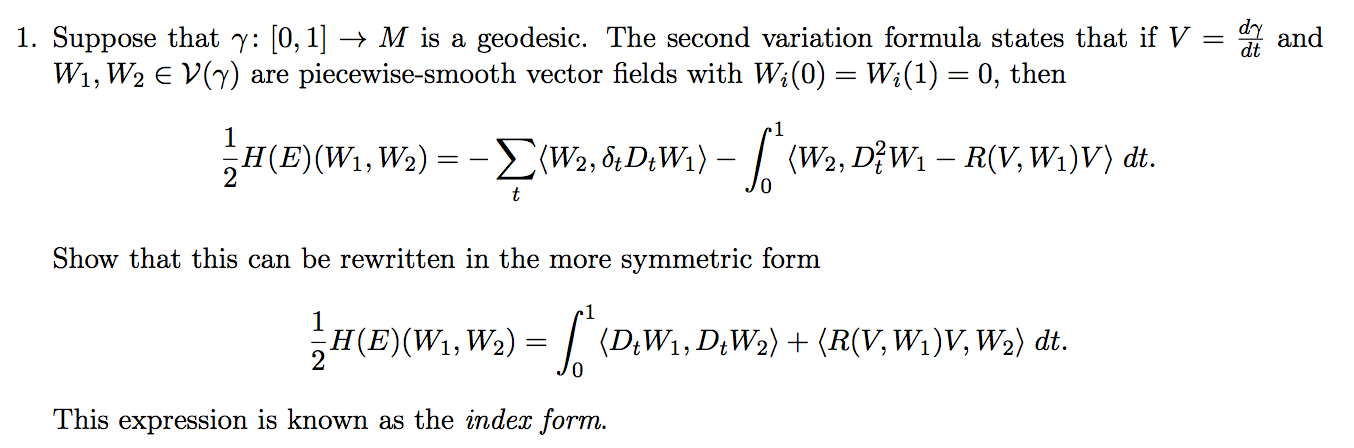
\includegraphics[width=0.7\textwidth]{dg-s5-p1.png}
\end{figure}
\end{question}
\begin{solution} \hfill \\
From
\eQb
\dfrac{d}{dt} <W_2, D_t W_1> &=& 
-<D_tW_1, D_t W_2> + <W_2, {D_t}^2 W_1>  
\eQe
it follows that
\eQb
\dfrac{1}{2} H(E)(W_1, W_2) &=& = - \sum_{i} <W_2, \triangle_{t} D_t W_1> 
- \int_{0}^{1} <W_2, D_t^2 W_1 - R(V,W_1)V> dt \\
&=&  -\sum_{i} \int_{t_{i-1}}^{t_i} (\dfrac{d}{dt}<W_2, D_t W_1>) dt 
+ \int_{0}^{1} <W_2, D_t^2 W_1> + <R(V,W_1)V, W_2> dt \\
&=& \int_{0}^{1} <D_t W_1, D_t W_2> + <R(V,W_1)V,W_2> dt. 
\eQe
\hfill $\qed$
\end{solution}

\newpage

\begin{question}[1-2]
\hfill
\begin{figure}[h!]
  \centering
    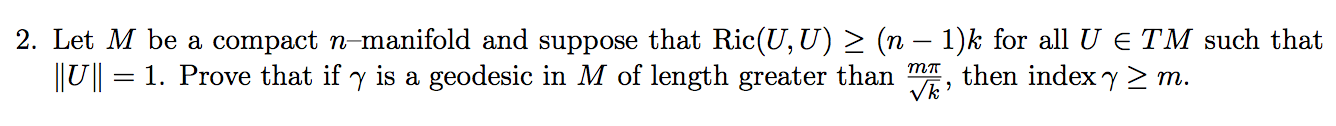
\includegraphics[width=0.7\textwidth]{dg-s5-p2.png}
\end{figure}
\end{question}
\begin{solution} \hfill \\
From the given Ricci lower bound, we see that the hypothesis of Myer's theorem is 
satisfied with the positive constant $\frac{1}{\sqrt{k}}$, and hence 
any geodesic $\gamma$ with length greater than $\frac{\pi}{\sqrt{k}}$ contains
conjugate points, which implies that the index of $\gamma$ is at least $1$. We now
proceed by induction. Suppose the statement is true for some $m  > 1$. Then, 
split a geodesic $\gamma$ with length greater than $\frac{(m+1)\pi}{\sqrt{k}}$ 
into two parts where $\gamma_1$ has the length 
greater length $m\frac{\pi}{\sqrt{k}}$, and $\gamma_2$ has the length greater than
$\frac{\pi}{\sqrt{k}}$. Then, by Morse Index theorem, and the inductive hypothesis
\eQb
\text{Index}(\gamma) &=& 
\sum_{q \> \text{conjugate to } p; \> q \in \gamma((0,1])} 
Ord(q) \\
&\geq&
\sum_{q \> \text{conjugate to } p; \> q \in \gamma_1((0,1])} 
Ord(q) \geq m \\
\eQe 
where $p = \gamma(0) = \gamma_1(0)$. Hence, it suffices to show that there is a 
conjugate point to $p$ along $\gamma_2$. Now, as $\gamma_2$ has length greater than
$\frac{\pi}{\sqrt{k}}$, we know that there is a point on the image of $\gamma_2$
such that it is conjugate to $\gamma_2(0)$. Hence, it now suffices to show the following:
let $p,q,r$ be $p = \gamma(0), q = \gamma(t_1)$, and $r = \gamma(t_2)$, such that
$0 < t_1 < t_2$, and
$r$ is conjugate to $q$. Then, there exists $t^* \in [t_1,t_2]$ such that 
$\gamma(t^*)$ is conjugate to $p$. The statement is true, since if $r$ is conjugate
to $q$, then the index along the geodesic from $p$ to $r$ must increase from
$q$ to $r$, by monotonicity, so using Morse theorem one more time,
 we are done. \hfill $\qed$
\end{solution}

\newpage

\begin{question}[1-3]
\hfill
\begin{figure}[h!]
  \centering
    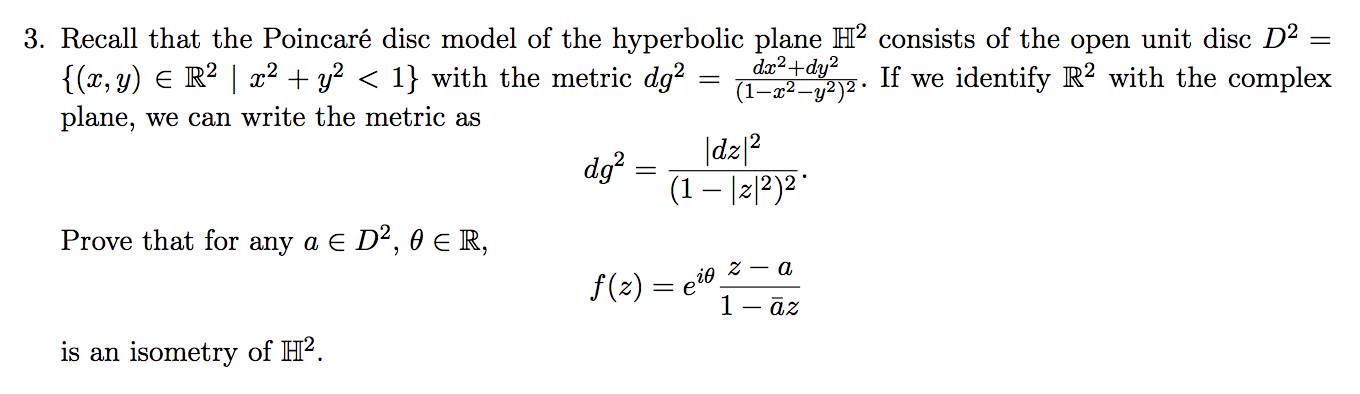
\includegraphics[width=0.7\textwidth]{dg-s5-p3.png}
\end{figure}
\end{question}
\begin{solution} \hfill \\
Using the isometry between the upper half plane model and the ball model, $\dfrac{
zi+1}{z+i}$, we can instead argue that $z \mapsto \dfrac{az+b}{cz+d}$ for any
$a,b,c,d \in \mathbb{R}$ with $ad - bc = 1$, is an isometry on $\mathbb{H}^2$. Now,
it suffices to show that for any piecewise differentiable path in $\mathbb{H}^2$,
$\gamma:I \to \mathbb{H}^2$, $L(\gamma) = L(f(\gamma))$, as this will determine
the hyperbolic distance. Set $z(t) = (x(t),y(t))$ and $w(t) = f(z(t)) = u(t) + iv(t)$.
Then,
\eQb
\dfrac{dw}{dz} &=& \dfrac{a(cz+d) - c(az+b)}{(cz+d)^2} = \dfrac{1}{(cz+d)^2} 
\eQe
and
\eQb
v &=& Im(w) = \dfrac{w - \bar{w}}{2i} = \dfrac{Im(z)}{|cz+d|^2} = \dfrac{y}{|cz+d|^2}.
\eQe
Hence,
\eQb
\left| \dfrac{dw}{dz} \right| &=& \dfrac{v}{y}
\eQe
and
\eQb
L(f(\gamma)) &=& \int_{0}^{1} \dfrac{|\frac{dw}{dt}|}{v(t)} dt = 
\int_{0}^{1} \dfrac{|\frac{dw}{dz} \frac{dz}{dt}|}{v(t)} dt = 
\int_{0}^{1} \dfrac{|\frac{dz}{dt}|}{y(t)} dt = L(\gamma), 
\eQe
as required. \hfill $\qed$

\end{solution}

\end{document}


